\title{Independent Research: History of The Proton Radius Puzzle}
\author{
        Ethan Rooney \\
                Department of Physics\\
        George Washington Univerisity\\
        Washington D.C., 20052
}
\date{\today}

\documentclass[12pt]{article}
\usepackage{array}
\newcolumntype{L}{>{\centering\arraybackslash}m{1.8cm}}
\usepackage{amsmath}
\usepackage{graphicx}
\usepackage{epigraph}
\graphicspath{ {.images/} }

\begin{document}
\maketitle

%\begin{abstract}
%\end{abstract}

%\section{Introduction}
%(Draft, don't worry about this)
%In this paper I am writing for a 2nd year undergraduate student.
%I am trying to give them the tools they need to on ramp into proton radius research.
%The major highlights are:
%Rutherford Scattering;
%Discovery of the proton; 
%Using Electrons to scatter off of hydrogen targets;
%Breakdown of Rutherford differential cross-section at relativistic speeds;
%N. F. Mott relativistic speeds;
%Divergence from Mott Curve;
%Form Factors;
%Electron Scattering experiments;
%Electron spectroscopy;
%Muon Spectroscopy;
%Muon Scattering;
%MUSE

\section{Rutherford Scattering}

In 1908, a plum-pudding model of the atom was one of the leading explanations of atomic behavior.
This plum-pudding model had a diffuse cloud of positive charge, spread over the whole range of the influence of the atom ~$10^{-10}$ meters, with negative charges embedded inside. 

Dr. Ernest Rutherford enlisted the help of Dr. Hans Geiger and an undergraduate assistant, Ernest Marsden, in probing the structure of the atom.

In 1908 Geiger, Marsden and Rutherford had shown that $\alpha$ particles would undergo a small deflection, typically less than $1^\circ$ when passing through a metal foil\cite{Geiger1908}.
This result was in agreement with the expected behavior of the plum pudding model.

Following that experiment Geiger and Rutherford tasked Marsden with creating a new experiment.
He was to check for $alpha$ particles deflected back towards the source of the $alpha$ particles.
The senior scientists expected no significant results.

In this new experiment Marsden the measured for large angle deflections, especially those particles scattering at greater than $90^\circ$.

\begin{figure}[h]
    \centering
    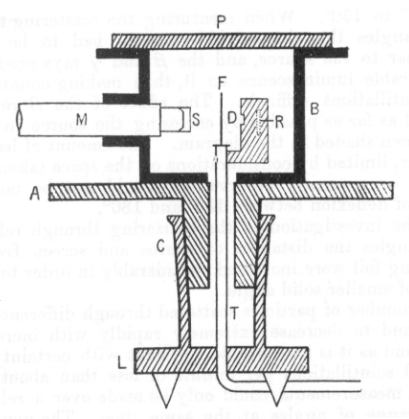
\includegraphics[width=7cm]{gold_foil_device}
    \caption{Geiger-Marsden $\alpha$ scattering device\cite{Geiger1913}}
    \label{fig:device}
\end{figure}


In Figure \ref{fig:device} we see a cross section of the device used to gather the distribution of $\alpha$ particles scattered from a thin metal foil.
The device consisted of an evacuated box B, inside of which there was a Radium $\alpha$ source R, and a gold foil F.
Between the $\alpha$ source and foil was a collimating diaphragm D.
This diaphragm only allowed a small "pencil of $\alpha$ particles" to be incident on the foil.
The experimenter could then look at the screen S coated in a substance that would let out a pulse of light, in a processes known as scintillation, when struck by a charged particle.
This scintillation screen was attached to the end of microscope M.
The microscope and scintillation screen could be rotated around the foil and $\alpha$ source, allowing for the experimenter to collect events at an arbitrary scattering angle. 
Whenever a scattered particle deflected into the observed angle,the scintillator coating would light up. Marsden would tally each of these scintillations by hand.
For several of the experiments, Geiger and Marsden collected data from 5 degrees to 150 degrees off of the beam line.
This data allowed them to quantify the differential cross section, or the number of scattering events that occur as a function of the scattering angle.
They found $1$ in $8$ thousand events underwent a large deflection. 
These backscatters, were significantly less likely to occur than the those at lesser angles, never the less they could be observed.

We can see the some of the data they collected for an experiment run with both a gold foil and a silver foil in Table \ref{table:gvs}.

\begin{table}[h]
    \begin{tabular}{|L|L|L|L|L|L|}
        \hline
          &  & \multicolumn{2}{c|}{Silver Foil} &\multicolumn{2}{c|}{Gold Foil} \\ \cline{3-6}
        Angle of deflection $\phi$ & $\frac{1}{\sin^4{\phi/2}}$ & Number of Scintillations, $N$ & $\frac{N}{\sin^4{\phi/2}}$ & Number of Scintillations, $N$ & $\frac{N}{\sin^4{\phi/2}}$\\
        \hline
        150&1.15&22.2&19.3&33.1&28.8\\
        135&1.38&27.4&19.8&43.0&31.2\\
        120&1.79&33.0&18.4&51.9&29.0\\
        105&2.53&47.3&18.7&69.5&27.5\\
        75&7.25&136&18.8&211&29.1\\
        60&16.0&320&20.0&477&29.8\\
        45&46.6&989&21.2&1435&30.8\\
        37.5&93.7&1760&18.8&3300&35.3\\
        30&223&5260&23.6&7800&35.0\\
        22.5&690&20300&29.4&27300&39.6\\
        15&3445&105400&30.6&13200&38.4\\
        \hline
    \end{tabular}
    \caption{Original Data as reported by Geiger and Rutherford \cite{Geiger1913}}
    \label{table:gvs}
\end{table}

\begin{samepage}
\begin{quote}
    It was quite the most incredible event that has ever happened to me in my life. It was almost as incredible as if you fired a 15-inch shell at a piece of tissue paper and it came back and hit you.
\end{quote}
\begin{flushright}
    ---Rutherford\cite{roller1958}\\
    Upon Hearing the results of Marsden's Research
\end{flushright}
\end{samepage}

This plum pudding model had a problem.
In order for a charged particle to undergo a backscatter, the particle has to loose all of its forward momentum, slow to a stop in the direction of the beam and then turn back towards the source.
An $\alpha$ particle emitted by a decay of radium carries ~$4.87$ MeV of energy.
This is the electrostatic potential energy that must be reached by the $\alpha$ particle while transiting the nucleus in order to be backscattered.
If the positive charge is distributed over the whole region of the atom as required by the plum pudding model, then the electric field formed by the nucleus would be as described in Equation \ref{eq:efield-diffuse}.

\begin{equation}\label{eq:efield-diffuse}
    E = \frac{kQr}{R^3}\hat{r}
\end{equation}

Where k is the coulomb constant, Q is the charge of the atom, r is the distance from the center of the atom, and R is the radius of the atom \cite{Rutherford1911}.
Using Equation \ref{eq:efield-diffuse} we can find the electrical potential and thus the potential energy of an $\alpha$ particle traveling inside the atom.

\begin{equation}
    \Delta{V} = V(R)-V(r) = -\int_r^RE\cdot{ds} = -\int_r^RE dr = \frac{-kQ}{R^3}\int_r^Rr dr
\end{equation}

\begin{equation}\label{eq:potential-diffuse}
    V(r) = \frac{kQ}{2R}(3-\frac{r^2}{R^2})
\end{equation}

Since the potential of a charged particle is given by $V\cdot{q}$ we can find the potential energy of a particle traversing the plum-pudding nucleus, as seen in Figure \ref{fig:plumenergy}

\begin{figure}
    \centering
    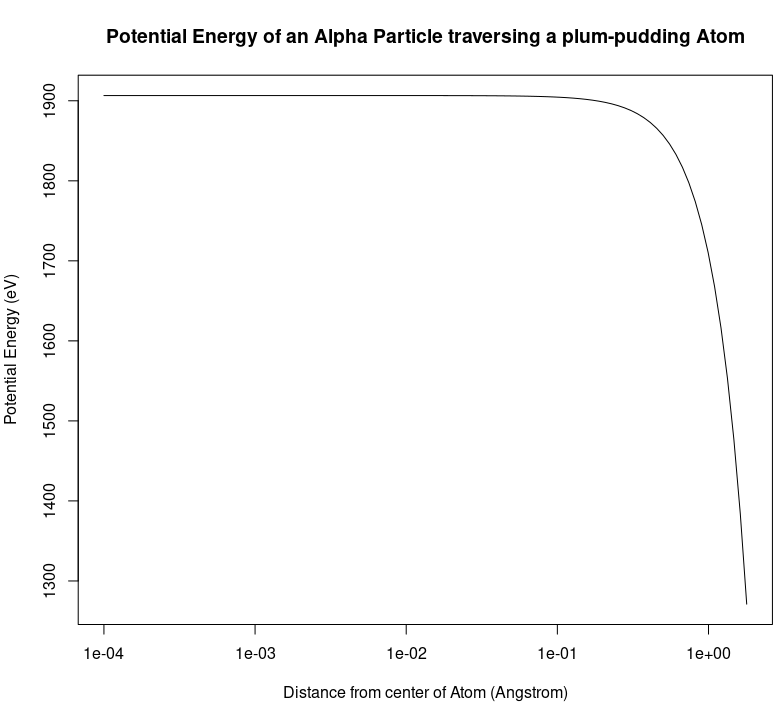
\includegraphics[width=10cm]{plumenergy}
    \caption{The Plum-Pudding model of an atom cannot generate the forces required to turn an $\alpha$ particle through a large angle}
    \label{fig:plumenergy}
\end{figure}

According to the leading physics of the time, backscatter of $\alpha$ particles from a thin gold foil was something that wasn't supposed to be possible.
The energy carried by alpha particles should allow them to punch right through the atoms of gold with only a tiny deflection.
Most of the time, that is exactly what was observed.
$\alpha$ particles would pass through the foil with just the smallest of deflections ~$0.87^\circ$, but one out of every 20 thousand $\alpha$ particles would undergo a backscatter in a gold\cite{Rutherford1911}.
The electric field of the plum-pudding model was not sufficient to backscatter the charged particles.

Rutherford, continued exploring this with another newly discovered particle, the $\beta$ particle.
From other experiments, he knew that the $\beta$ the opposite charge of the $\alpha$, but when fired into a gold foil, they behaved similarly.
Most $\beta$ particles passed through the foil, but some would experience a large deflection \cite{Rutherford1911}.

In order to solve this discrepancy Rutherford proposed a different model for the charge distribution inside the atom. 
The model he suggested is the model we are broadly familiar with today. A small dense object with a central positive charge surrounded by orbiting electrons on the outside.
He also knew that, because of the charges involved, the electric field would only play a significant role if the $\beta$ particles penetrated inside of the electron layer. 
This result can be shown from Gauss's law in Equation \ref{eq:gauss}.

\begin{equation}\label{eq:gauss}
    \Phi_E = \frac{Q}{\varepsilon_0}
\end{equation}

In \ref{eq:gauss} $\Phi_E$ is the electric flux through a closed surface, $Q$ is the total charge, and $\varepsilon_0$ is the electric constant.
Since the net charge of an atom is neutral, the $\Phi_E$ must be zero until you get inside of the electrons of the atom.

Given this information we can see that the electric field and Electric potential must be as we see in Equations \ref{eq:potential} and \ref{eq:electricfield}

\begin{equation}\label{eq:potential}
V = Ne(\frac{1}{r} - \frac{3}{2R} + \frac{r^2}{2R^3})
\end{equation}

\begin{equation}\label{eq:electricfield}
E = -\frac{dV}{dr} = Ne(\frac{1}{r^2} - \frac{r}{R^3})
\end{equation}

Where V is the electric potential, E is the electric field, r is the distance from the center of the atom, R is the Radius of the electron orbits, k is the Coulomb constant, N is the Atomic Number, e is the elemental charge.

In the equation for the electric field above, the positive contribution is from the central charge, and the negative term is from the electrons surrounding it.
With this new model the field attains a strength high enough to turn some incoming particles around, while allowing for most particles coming in to undergo a relatively small deflection.

It is illustrative to look at how an $\alpha$ particle fired directly at the nucleus would behave. $\alpha$ particle fired directly at the central charge, with some velocity $v$, would carry the energy in Equation \ref{eq:KE}.

\begin{equation}\label{eq:KE}
    KE = \frac{1}{2}mv^2
\end{equation}

From a conservation of energy standpoint, the particle would have to come to a complete stop when the potential energy of system was equal to the initial kinetic energy.
Given that the potential energy of a charged particle in a electric potential can be found with Equation \ref{eq:electricPE}.

\begin{equation}\label{eq:electricPE}
    PE = Vq = qNe(\frac{1}{r^2} - \frac{r}{R^3})
\end{equation}

Substituting Equation \ref{eq:KE} into Equation \ref{eq:electricPE} we get Equation \ref{eq:KEPE} below.

\begin{equation}\label{eq:KEPE}
    \frac{1}{2}mv^2 =  qNe(\frac{1}{r} - \frac{3}{2R} + \frac{r^2}{2R^3})
\end{equation}

Assuming r is very small compared to R when the particle stops, Equation\ref{eq:KEPE} can be simplified to Equation \ref{eq:KEPEsimple}

\begin{equation}\label{eq:KEPEsimple}
    \frac{1}{2}mv^2 = qNe(\frac{1}{r} - \frac{3}{2R})
\end{equation}

As we can see in the graph below, the Potential energy of a particle very close to the center of an atom is extremely high, but for most particles passing through an atom, the forces they experience will be relatively small, causing only a small deflection.

\begin{figure}
    \centering
    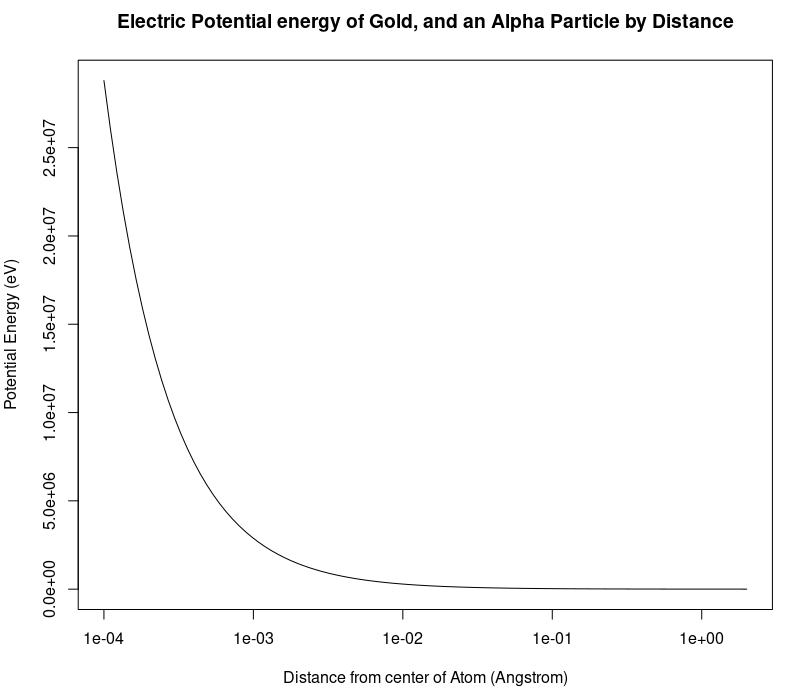
\includegraphics[width = 10cm]{ruthenergy}
    \caption{Potential Energy of a $\alpha$ particle as a function of the distance from the nucleus.}
    \label{fig:ruthenergy}
\end{figure}

Thus we find the particle will come to rest when $r=[\frac{2qNe}{mv^2} + \frac{3}{2R}]^{-1}$.
This stopping distance, $b$, is important for predicting the differential cross-section expected from a point nucleus.


As we can see in Figure \ref{fig:ruthenergy} the energy of a charged particle increases rapidly if the nucleus is sufficiently dense. This high central density makes it possible for backscattering to occur.

While $\alpha$ particles are useful in probing the structure of large atoms, they have an atomic mass of approximately $4$ amu.
This means that for probing the structure of small atoms, we can no longer make the assumption that no momentum is transferred into the target nucleus.
Additionally, when an $\alpha$ particle gets close to the target nucleus, the short range nuclear forces are no longer negligible.
Fortunately, $\beta$ particles had neither of these draw backs.
Electrons, and leptons broadly, are particles that cannot interact with the nuclear forces, and will only interact through coulomb forces, and therefore are able to be used in place of $\alpha$ particles for probing deeper into the nucleus.
These $\beta$ particles also known as electrons, have a rest mass of of $5.45*10^-4$ amu.


In 1920 Rutherford made another discovery fundamental to nuclear physics. He showed that when nitrogen gas was bombarded with $\alpha$ particles hydrogen gas was generated.

From this he was able to conclude that the positive charges in every atom were the same as that present in hydrogen gas\cite{Rutherford1920}.
It was at this point that physicists turned their attention to measuring this basic building block.

\begin{equation}\label{eq:proton_disc}
    N_{14} + \alpha \rightarrow O_{17} + p
\end{equation}

\section{Proton Radius, N.F. Mott, Relativity, and Dirac}

If the particle at the center of a hydrogen atom was a point particle, we would expect the follow Rutherford's formula for differential cross-section Equation \ref{eq:rutherforddifcross}, at least for non-relativistic scattering \cite{Hofstadter1956}.

Because Rutherford's differential cross section equation \ref{eq:rutherforddifcross} breaks down at higher energies, it couldn't be used to distinguish a highly compact object or one that was a point particle. For that we can turn to the theoretical work of N. F. Mott.

Mott expanded upon the work of Rutherford and extended Equation \ref{eq:rutherforddifcross} into a relativistic regime\cite{Hofstadter1956}.

\begin{equation}\label{eq:rutherforddifcross}
    \sigma(\theta) = \frac{q^2Q^2e^4}{16E^2\sin^4(\frac{\theta}{2})}
\end{equation}

\begin{equation}\label{eq:mottscatter}
    \sigma_M(\theta) = (\frac{Ze^2}{2mc^2})^2(\frac{1-\beta^2}{\beta^4})\frac{1}{\sin^4{\frac{\theta}{2}}}(1-\beta^2\sin^2\frac{\theta}{2})
\end{equation}

With this new relativistic model Mott could now make very precise predictions on the behavior higher energy electrons scattered from a point particle, and experimentalists like Hofstadter had new experiments to test those predictions. 

McAllister and Hofstadter constructed an experiment to test these new predictions of the behaviour of electron-proton scattering.
Rather than rely upon the decay of radioactive elements to produce charged particles as Rutherford had done, McAllister and Hofstadter utilised a particle accelerator to test the differential scattering cross section for 3 distinct energies, $100$, $188$ and $236$ MeV.
At 100 MeV, the Mott Curve is in broad agreement with the Rutherford Scattering, and so it was a control run to verify the experimental setup, at the higher energies the Mott curve diverges from Rutherford Scattering.

\begin{figure}
    \centering
    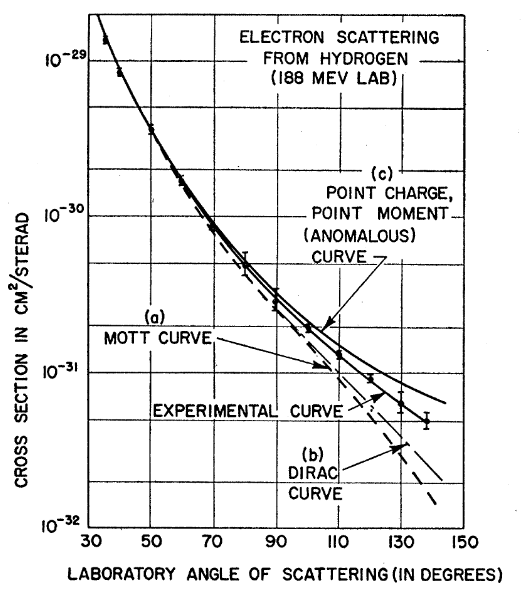
\includegraphics[width = 10cm]{mott_dirac_188mev}
    \caption{Holfstadter's 188MeV-electron scattering Experiment shows a deviation from the expected differential cross section of several theoretical models including the Mott Curve.}
    \label{fig:ruthenergy}
\end{figure}

The data collected by McAllister and Hofstadter diverged from any of the point particle experimental models, even those that had corrective terms accounting for the spin of the proton and electron, as well as the magnetic moment of those particles.

This deviation from predictions indicated that the electron was spending time inside of the proton, thus reducing the coulomb forces experienced between the proton and electron.
This was indication that the proton was of finite size.
What remained was to quantifying that size.

Rosenbluth had further extended the Mott-Rutherford differential cross-section equation or use in a quantum system. See Equation \ref{eq:rosenbluth} for the cross-section of a diffuse proton\cite{McAllister1956}.

Equation \ref{eq:rosenbluth_point} is the differential cross-section we would expect from a proton that was a point particle. 

\begin{equation}\label{eq:rosenbluth_point}
\sigma = \sigma_{NS}[1 + \frac{Q^2}{4M^2}[2(1+\mu)^2*\tan^2(\theta/2)+\mu^2]]
\end{equation}

Where $\sigma_{NF}$ was found with Equation \ref{eq:sigmanf} and \ref{rosenbluth_Q}.

\begin{equation}\label{eq:sigmanf}
    \sigma_{NS} = \frac{e^4}{4E^2}(\frac{\cos^2(\theta/2)}{sin^4(\theta/2)}\frac{1}{1+(2E/M)sin^2(\theta/2)})
\end{equation}

\newcommand{\lambdabar}{{\mkern0.75mu\mathchar '26\mkern -9.75mu\lambda}}

\begin{equation}\label{rosenbluth_Q}
    Q = \frac{(2/\lambdabar)\sin(\theta/2)}{[1+(2E/M)sin^2(\theta/2)]^\frac{1}{2}}
\end{equation}

Were $\lambdabar$ is the reduced De Brogli wavelength. $E$ is the kinetic Energy of the electron beam. $M$ is the mass of the electron and $\theta$  is the scattering angle. $Q$ is the invariant momentum transfer in the Center of Mass frame.

If however the proton was not a point particle and indeed has some distorbution of charge, Equation \ref{eq:rosenbluthdiffuse}.

\begin{equation}\label{eq:rosenbluthdiffuse}
    \sigma = \sigma_{NS}[F_1^2 + \frac{q^2}{4M^2}[2(F_1+\mu{F_2})^2*\tan^2(\theta/2)+\mu^2F_2^2]]
\end{equation}

Where $F_1$ and $F_2$ were the form factors of the electric cahrge and magnetic moment distrobution. While they are not required to be the same, they are often treated as equal.

Using this method McAllister and Rosenbluth were able to measure the proton radius to be $.74 \pm 0.24$ fermi .

\bibliographystyle{plain}
\bibliography{simple}

\end{document}
  
